\documentclass[lettersize,journal]{IEEEtran}
\usepackage{amsmath,amsfonts}
\usepackage{algorithmic}
\usepackage{array}
\usepackage[caption=false,font=normalsize,labelfont=sf,textfont=sf]{subfig}
\usepackage{textcomp}
\usepackage{stfloats}
\usepackage{url}
\usepackage{verbatim}
\usepackage{graphicx}
\usepackage{cite}
\graphicspath{ {./plots/} }
\def\BibTeX{{\rm B\kern-.05em{\sc i\kern-.025em b}\kern-.08em
    T\kern-.1667em\lower.7ex\hbox{E}\kern-.125emX}}
\usepackage{balance}
\begin{document}
\title{Q-learning in the snake game}
\author{Adam Zaiter}

\maketitle

\begin{abstract}
\end{abstract}

% \begin{IEEEkeywords}
% \end{IEEEkeywords}


\section{Introduction}
This paper will attempt to implement the Q-learning algorithm
for a basic game of snake. A hypothesis about the expected learning
outcome will be established and reviewed after implementing the
Q-learing algorithm. The implementation will be done in Python
and a custom snake game environment will be created.
This environment will allow for training of the agent with different
hyperparameters as well as visualizing a game played by the
trained agent.


Basic knowledge of reinforcement learning is assumed, as this paper
is implementing concepts from the Szepesvari paper \cite{szepesvari}.

\section{Snake game}
The snake game is programmed in python.
It supports square grids of any size that is $>= 3$.
The snake starts in the middle of the grid with a head of
1 square in size and attached
body with 2 squares in size. There also is food spawned in a random
square that is not occupied by the snake. The objective for the
snake is to eat as much food as possible. If the food is eaten,
the snake gains + 10 score and grows an additional body part of
1 square in size. If the snake collides with the borders of the grid
or the head collides with it's own body, the game ends.\label{game-over}


\section{Q-learning}
Q-learning will be used as the algorithm to train the agent.
It finds the optimal policy by learning
the best Q values for each state-action pair.

The Q function accepts the current state and an action. It then
returns the expected reward for taking said action for the given
state.

The agent then plays episodes. For each step in the episode
the Q values in the Q table are updated using the Bellman
equation. This process goes on until the q function converges
to the optimal function q*.

\section{Hypothesis}
The goal is to train an agent that will play the snake game
with any chosen grid size as best as possible using just Q-learning.
Given the attributes of Q-learning, it should be possible to train
an agent that plays the game of snake at a very good level. It
is not expected to be perfect, but it should play as close to it
as possible.

\section{Environment}
The environment mimics functionality provided by environments in
OpenAI gyms \cite{openai}. This made the process of applying the Q-learning
algorithm quite simple, as the OpenAI environments are designed
with reinforcement learning in mind.

\subsection{Action space}

The environment provides three actions for the agent to take:
\begin{enumerate}
    \item Turn the snake head left.
    \item Turn the snake head right.
    \item Continue heading straight.
\end{enumerate}
These values are encoded as integers 0, 1, 2 and aliased as
constants LEFT, RIGHT and STRAIGHT in the code.


\subsection{State space}
For this project, the computing resources are somewhat limited and
as such, these limited resources have to be taken into consideration
when designing the state and action spaces.
The state space for a snake game with a variable size would be
too big, if it were taken as is. That is, because the snake and
it's body adds many additional states, as the snake can grow it's body to
be the same size as all of the squares in the grid. Also, the head is distinct
from the other body parts and would have to be accounted for in all of the states.

For these reasons the current environment does not provide the full state of the board. Thus, the environment is restricted to
this basic information:
\begin{itemize}
    \item Information about danger. It indicates if after taking an action from the action space in the current state
        the game will be over.
    \item Information about food position with respect to the snake's head. The values are left, right, up and down.
    \item Information about the snake's current direction. There are four values: left, right, up and down.
\end{itemize}

After gathering this information, it is encoded in a 2D array. For example, the array for food position
is an array of four values. Each position of the array corresponds to a value (left, right, up, down).
Thus if the food is left, the array on position left will have the value of 1 (true). Otherwise, the
value will be 0 (false). This applies for all positions. In the end, three individual arrays for danger,
food and direction are created and are returned concatenated as the current state.


\subsection{Extending the state space}
The most obvious way to extend the state is to add more
information about danger. For the most basic case, danger
is supplied as an array of boolean values. From the current
state a lookahead is performed on every action from
the actions space. If the action would result in a game
over, danger is set to true for that action. This
array can be extended to looking ahead more than one action
in the future. This however grows the danger array
exponentially, so the comparison in the coming experiments
will be made only between one and two future actions lookahead
(11 size state space and 20 size state space respectively).


\section{Training} \label{training}
The python program supports a training mode, where
training arguments can be provided. Some of those are the environment size,
total episodes to train for, decay rate, depth (size of state space),
learning rate and more.

The best results were observed in agents trained on the 3x3 grid environment.

All agents referenced below have been trained for 500 000 episodes
with an exponential decay rate with a value of 0.01. Minimum epsilon with value 0.01
was used to keep some exploration throughout the whole training
process.

Figure \ref{fig1} contains training statistics for the agent that was trained
with a limited information about danger. This agent performs well, however
it is unable to play perfect games very often at all.


% time python run.py --train --env_size 3 --o "3-depth.npy" --total_episodes 500000 --decay_rate=0.01 --depth
% time python run.py --train --env_size 3 --o "3-depth.npy" --total_episodes 500000 --decay_rate=0.01 --depth
\begin{figure}[!t]
\centering
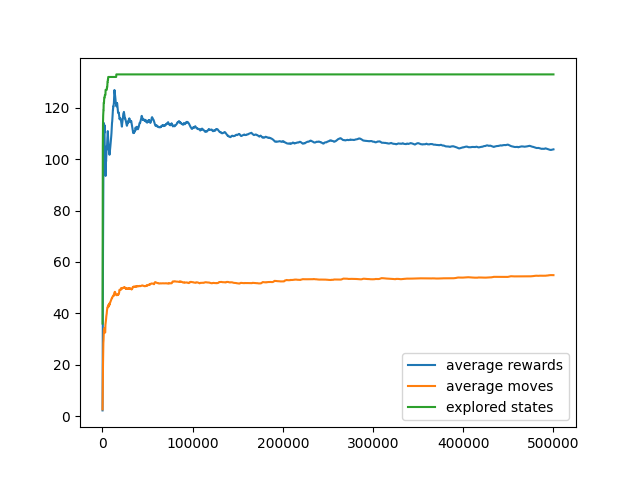
\includegraphics[width=3.5in]{3_fig.png}
\caption{3x3 environment 11-size state space}
\label{fig1}
\end{figure}

Figure \ref{fig2} show statistics for the agent that was trained on a
state space with information about danger for two turns ahead.
This agent performed considerably better than the previous agent and
is able to play a perfect game quite often on a 3x3 grid and on average outperforming
the aforementioned agent.

\begin{figure}[!t]
\centering
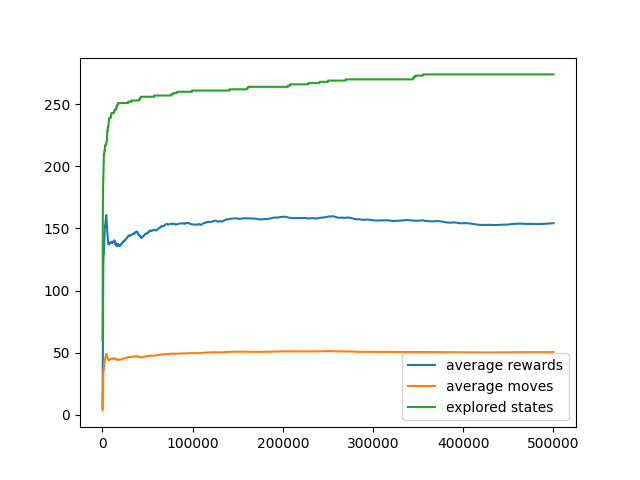
\includegraphics[width=3.5in]{3-depth_fig.png}
\caption{3x3 environment 20-size state space}
\label{fig2}
\end{figure}

\begin{figure}[!t]
\centering
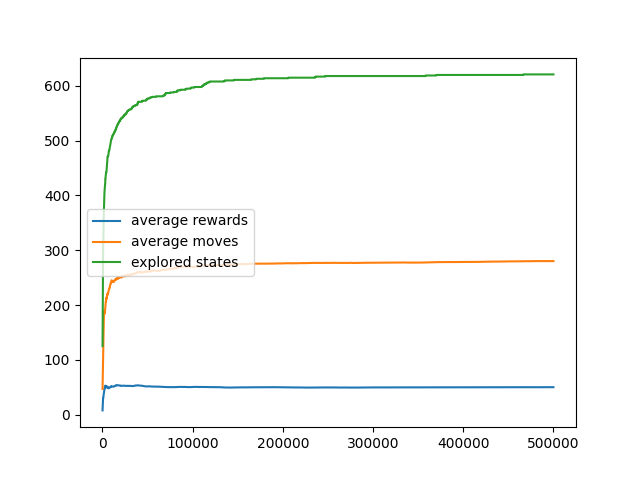
\includegraphics[width=3.5in]{16_fig.png}
\caption{16x16 environment 20-size state space}
\label{fig3}
\end{figure}


Finally, figure \ref{fig3} shows training of an agent on a 16x16 grid.
Expectedly, the performance is much worse than the other presented agents.

Both of the mentioned agents that were trained on a 3x3 grid are capable of playing games in larger environments with
reasonable performance. The agent trained on the larger state space continues
to outperform the other agent even in the larger environments.


\section{Observations}

\subsection{Learning}
The agent learns much better in smaller environments as evident from
the figures in section \ref{training}. One of the reason
undoubtedly is the amount of moves the agent has to make. In
smaller environments the number of moves made is much smaller,
allowing the agent to explore states and learn much quicker.
Another reason could be the amount of information the agent has
about the environment. In smaller environments the state space
looks much more similar to the real state of the game than in
larger environments.

Even with limited information the snake learns the strategy
of creating as much space as possible for it's own body.
This results in the snake hugging the borders as much
as possible, thus it takes longer paths to get to the reward (food) which
might seem strange early in the game.
However, when the snake's body is longer after collecting a
few rewards, the benefits of this strategy are fully visible.

Another interesting fact that can be observed from the training plots is
the dip in average rewards when new states are explored. This dip
is more significant for the agent with limited state space.


\subsection{Rewards}
Since the environment is custom, rewards had to be assigned for
performing certain actions. There are three types of reward
\begin{itemize}
    \item Reward for eating food.
    \item Cost for achieving game over state.
    \item Survival reward for making a move that did not result
        in game over.
\end{itemize}

Survival reward did not seem to make any significant difference.
Only when it was set too high the agent prefered to just move
around safely without picking up food.

A lot of experiments were conducted to find the right combination
of cost and reward. The one that seems to work most reasonably
is to have the cost to be negative double of the amount of the reward.

\section{Better algorithms for the snake game}
\begin{itemize}
    \item Function approximation - deep q learning.
    \item Hamiltonian cycle.
\end{itemize}

\section{Conclusion}


\begin{thebibliography}{1}
\bibitem{szepesvari}
    Csaba Szepesvari - Algorithms for Reinforcement Learning. [online] Available at: \url{https://sites.ualberta.ca/~szepesva/papers/RLAlgsInMDPs.pdf} [Accessed 15 January 2022].
\bibitem{openai}
    Open AI Gym. [online] Available at: \url{https://gym.openai.com/} [Accessed 15 January 2022].


\end{thebibliography}


\end{document}
